\documentclass[tikz]{standalone}

\usepackage{tikz}

\begin{document}

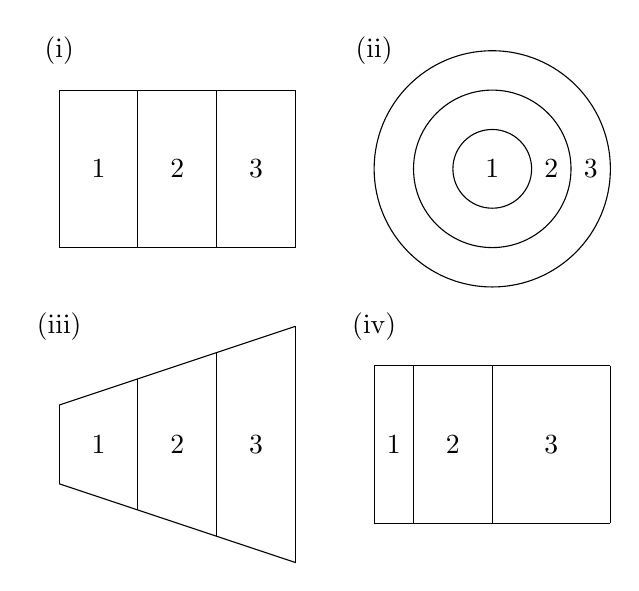
\begin{tikzpicture}
\node[] at (-1, 1.5) {(i)};nonumber
\node[] at (-0.5, 0) {1};
\node[] at (0.5, 0) {2};
\node[] at (1.5, 0) {3};
\draw (-1,1) -- (2,1);
\draw (-1,-1) -- (2,-1);
\draw (-1,-1) -- (-1,1);
\draw (2,-1) -- (2,1);
\draw (0,-1) -- (0,1);
\draw (1,-1) -- (1,1);

\node[] at (3, 1.5) {(ii)};
\node[] at (4.5, 0) {1};
\node[] at (5.25, 0) {2};
\node[] at (5.75, 0) {3};
\draw (4.5,0) circle (.5);
\draw (4.5,0) circle (1);
\draw (4.5,0) circle (1.5);

\node[] at (-1, -2) {(iii)};
\node[] at (-0.5, -3.5) {1};
\node[] at (0.5, -3.5) {2};
\node[] at (1.5, -3.5) {3};
\draw (-1,-3) -- (2,-2);
\draw (-1,-4) -- (2,-5);
\draw (-1,-4) -- (-1,-3);
\draw (2,-5) -- (2,-2);
\draw (0,-0.8333 - 3.5) -- (0,0.8333 - 3.5);
\draw (1,-1.1666 - 3.5) -- (1,1.1666 - 3.5);

\node[] at (3, 1.5 - 3.5) {(iv)};nonumber
\node[] at (3.25, 0 - 3.5) {1};
\node[] at (4, 0 - 3.5) {2};
\node[] at (5.25, 0 - 3.5) {3};
\draw (3,1 - 3.5) -- (6,1 - 3.5);
\draw (3,-1 - 3.5) -- (6,-1 - 3.5);
\draw (3,-1 - 3.5) -- (3,1 - 3.5);
\draw (6,-1 - 3.5) -- (6,1 - 3.5);
\draw (3.5,-1 - 3.5) -- (3.5,1 - 3.5);
\draw (4.5,-1 - 3.5) -- (4.5,1 - 3.5);

\end{tikzpicture}

\end{document}
